% !TEX root = main.tex

% \begin {table*}[tp]
\small
\begin{center} 
\vspace{-0. in}
\caption{Summary of Distributed Placement and Stacked-TLBs for Different
Performance Metrics}
\vspace{-0. in}
\begin{tabular}{| c | c | c | c | c | }
\hline
Metric & Baseline & Distributed & Stacked-TLB & Perfect-LLT \\
       &          &  Placement  &             &             \\\hline
\# Page Table Lookups/LLT miss  & 1.75 & 1.75 & 1.00 &0.00 \\\hline
\multicolumn{5}{|c|}{ } \\ \hline
\multicolumn{5}{|c|}{ 4KB Page Size} \\ \hline
Throughput                            & 1.00 & 1.28 & 1.44 & 1.96 \\\hline
Relative LLT Miss Latency             & 1.00 & 0.70 & 0.51 & 0.00 \\\hline
Relative LLC Miss Latency             & 1.00 & 1.07 & 1.11 & 1.10 \\ \hline
\multicolumn{5}{|c|}{ } \\ \hline
\multicolumn{5}{|c|}{ 64KB Page Size} \\ \hline
Throughput                            & 1.00 & 1.04 & 1.12  & 1.34 \\\hline
Relative LLT Miss Latency             & 1.00 & 0.85 & 0.61  & 0.00 \\\hline
Relative LLC Miss Latency             & 1.00 & 1.03 & 1.05  & 1.07 \\ \hline

\end{tabular}
\label{table:results_summary}
\vspace{-0.015 in}
\end{center}
\normalsize
\end{table*}


\section{Results and Analysis} 
\label{sec:result}

\subsection{Results Summary}

\begin{figure}[tp] 
\vspace{-0 in} \centering
\centerline{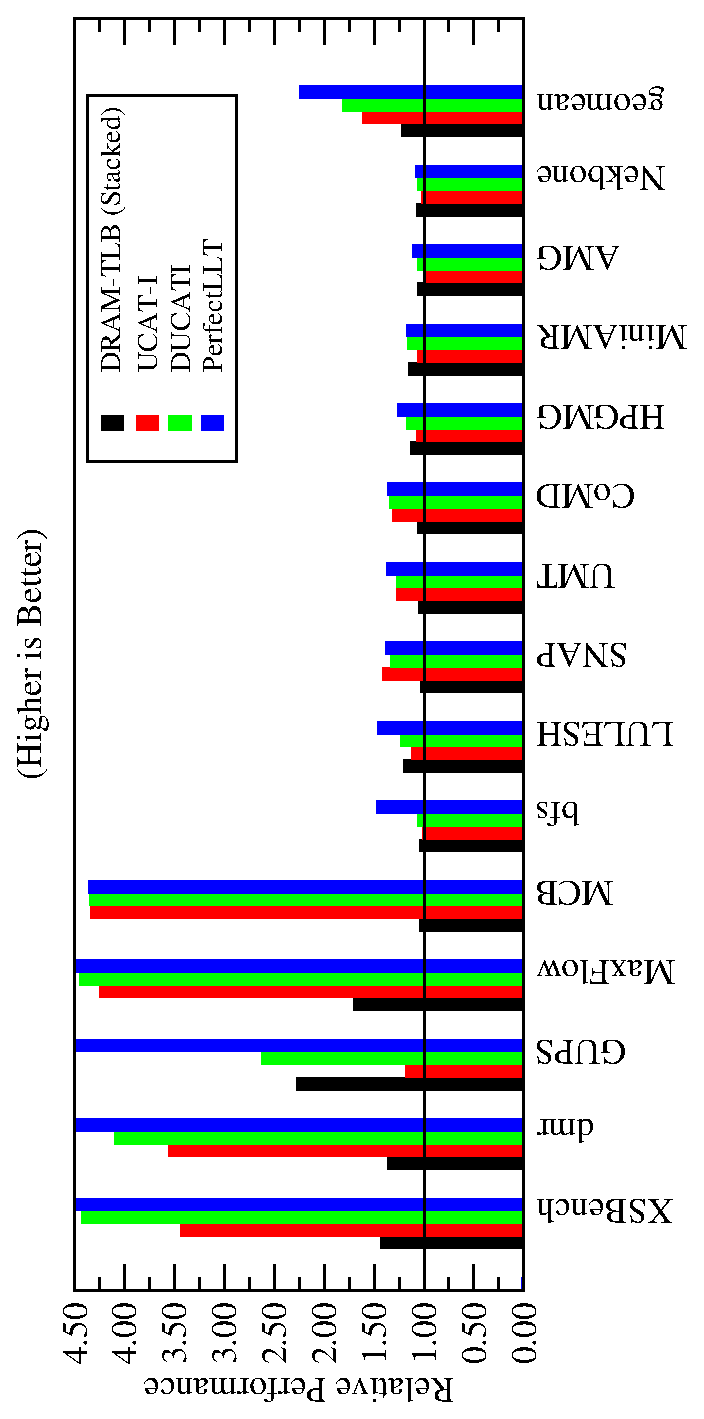
\psfig{file=GRAPHS/SUMMARY_perf,angle=-90,width=\columnwidth}}

\caption{\small Performance Summary (4KB page size).\normalsize}
\label{fig:summary_4k_pages} 
\vspace{0.1 in}
\end{figure}

\begin{figure}[tp] 
\vspace{-0 in} \centering
\centerline{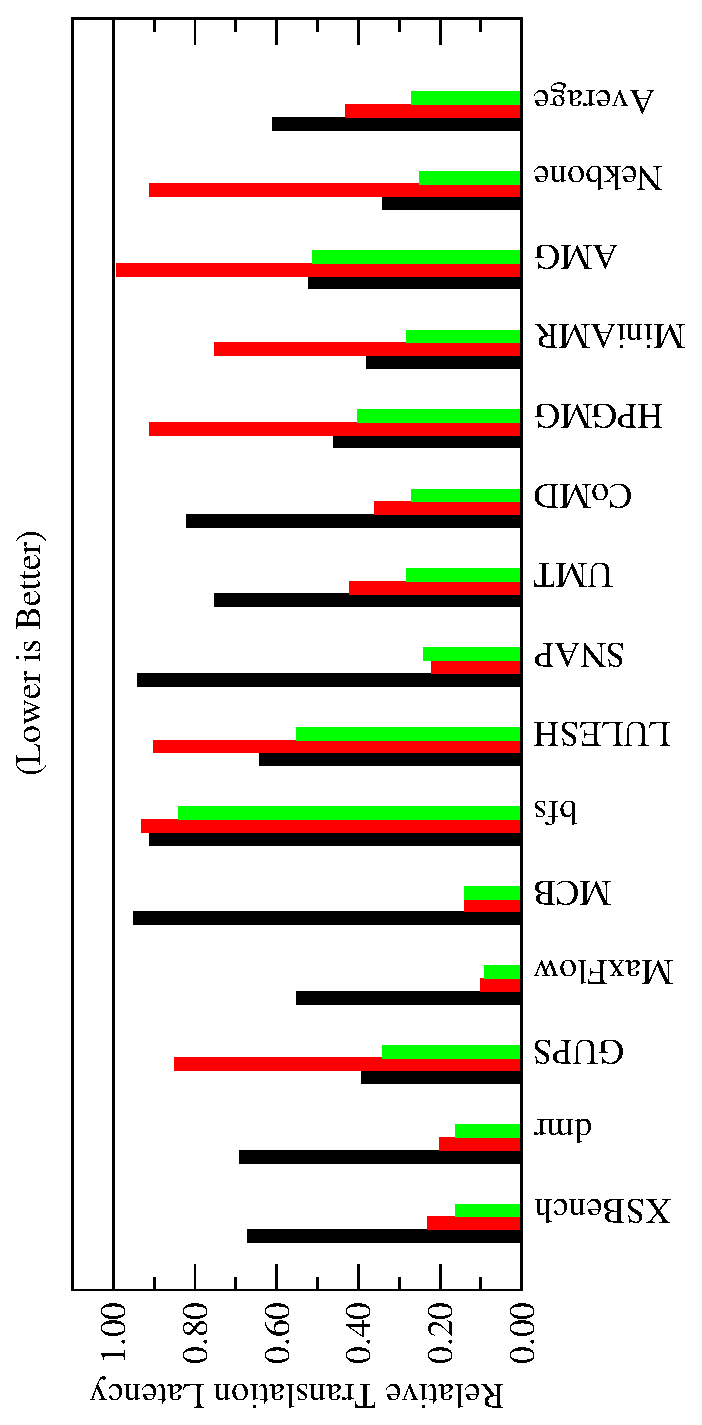
\psfig{file=GRAPHS/SUMMARY_tlblat,angle=-90,width=\columnwidth}}

\caption{\small Translation Latency (4KB page size).\normalsize}
\label{fig:summary_4k_pages} 
\vspace{-0. in}
\end{figure}

\subsection{Sensitivity to Page Size}

\noindent We now present the performance of our schemes using 64KB
page size. For our 1024-entry baseline LLT size, using 64KB pages
increases the TLB coverage to 64MB (up to 256MB because of
~\cite{COLT}). In doing so, the LLT miss frequency reduces for
workloads that have high spatial locality in the virtual address
space. Table~\ref{table:results_summary} summarizes the different
performance metrics relative to the baseline system. With 64KB page
size, Distributed Placement and Stacked-TLB reduce LLT miss latency by
15\% and 39\% respectively. In turn, they improve performance by 4\%
and 12\% respectively.

With 64KB page size, Figure~\ref{fig:summary_64k_pages} presents the
per workload performance behavior of our baseline system, Distributed
Placement and Stacked-TLB relative to a perfect LLT system. We observe
that workloads with high spatial locality within a 64KB page tend to
observe fewer LLT misses. Consequently, the baseline system itself is
within 30\% of a perfect LLT (as opposed to 50\% for the 4KB page size
system). However, there is still opportunity to improve performance of
workloads that are TLB-sensitive with 64KB pages (e.g. $HPGMG$, $DMR$,
and $XSBENCH$). For these workloads, Distributed Placement and
Stacked-TLB proposals improve performance by 27-45\%. Overall,
Stacked-TLB bridges 30\% of the performance gap between the baseline
system and a perfect LLT.


% However, for workloads with limited
% spatial locality in a 64KB page (e.g. HPGMG, DMR) still benefit from
% our proposals.
% 
% We show that that distributed pagetable placement improves performance
% by 4\% while DRAM-TLBs and Stacked-TLBs improve performance by 14\%
% and 11\% respectively. We find the performance benefits from
% distributed page table placement diminishing with increasing page
% size. This is beacause fewer LLT misses cause the average number of
% memory requests to the memory system to increase. Since the majority
% of requests are serviced by the stacked memory, increasing queuing
% delays take away any benefit realized from page table placement. 
% 
% We note that it is exactly for this reason that DRAM-TLBs also
% outperform Stacked-TLBs at times. Since the majority of requests are
% serviced by stacked memory, average stacked memory access latency can
% be longer than the average system memory access latency (at least
% until system memory bandwidth saturates).

\begin{figure}[tp] 
\vspace{0. in} \centering
\centerline{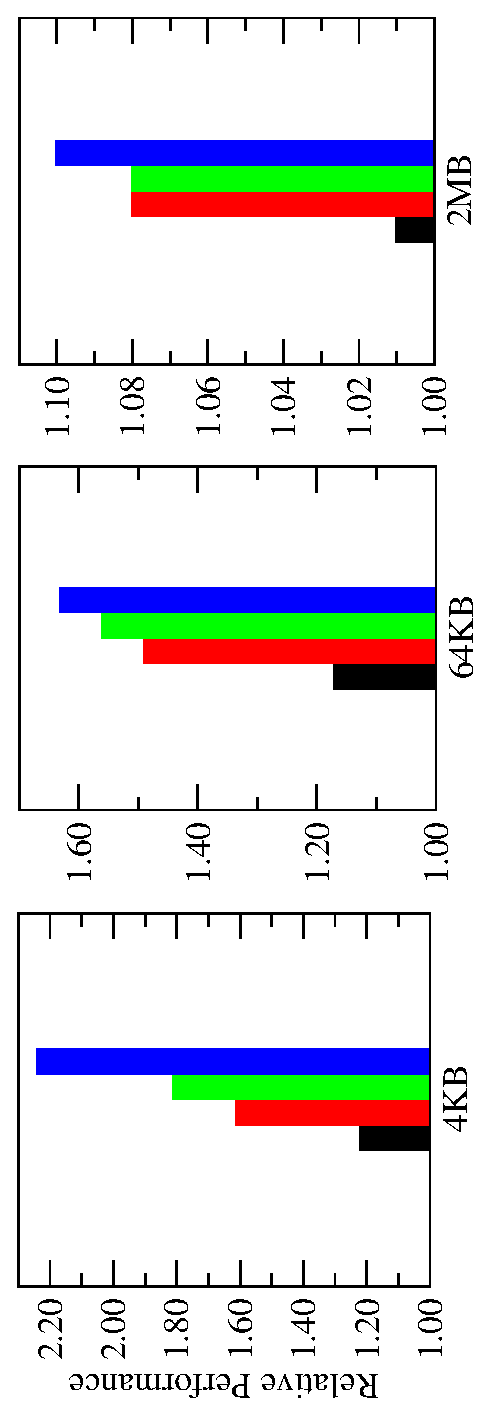
\psfig{file=GRAPHS/pagesize_sensitivity2,angle=-90,width=\columnwidth}}

\caption{\small Performance Sensitivity to Page Size.\normalsize}

\label{fig:summary_pagesize} 
\vspace{-0. in}
\end{figure}

% \subsection{Sensitivity to Stacked DRAM Bandwidth}
% 
% \noindent Figure~\ref{fig:stack_bw_sense} illustrates the sensitivity
% of our proposals to stacked memory bandwidth. We evaluate four
% additional systems with 0.25X, 0.5X, 2X, and 4X the stacked memory
% bandwidth of the baseline system (we do not vary the system memory
% bandwidth). We increased the bandwidth by increasing the number of
% channels in the stacked memory system. The y-axis illustrates the
% average performance relative to the baseline system across all
% workloads in the study.
% 
% The figure shows that when the stacked memory bandwidth is plentiful,
% our proposals continue to improve performance. However, when the
% stacked memory bandwidth becomes a bottleneck, the memory queuing
% delays limit the performance of Distributed Placement. Under such
% scenarios, Stacked-TLBs still improve performance since they reduce
% the number of memory references. In general, our proposals efficiently
% utilize the spare bandwidth available in the stacked memory system.
% When the available bandwidth is high, performance improvements are
% high. When the available bandwidth is low, performance improvements
% are low.
% 
% \begin{figure}[t] 
% \vspace{0.1 in} \centering
% \centerline{\psfig{file=GRAPHS/sensitivity_stack_bw,angle=-90,width=\columnwidth}}
% 
% \caption{\small Sensitivity to stacked memory bandwidth. \normalsize}
% \label{fig:stack_bw_sense} 
% \vspace{-0 in}
% \end{figure}
% 
